%%%%\%%%%%%%%%%%%%%%%%%%%%%%%%%%%%%%%%%%%%%%%%%%
%% Introduction aux Systèmes d'exploitation  %%
%%   * Historique                            %%
%%   * Principes fondamentaux                %%
%%   * Grandes classes de systèmes           %%
%%%%%%%%%%%%%%%%%%%%%%%%%%%%%%%%%%%%%%%%%%%%%%%

\title{Systèmes d'exploitation, 2ème année}
\subtitle{Multi-Threading}

\author{Yves \textsc{Stadler}}
\institute{Université de Lorraine - IUT de Metz}

\date{\today}

\begin{document}

%%
% Page de Titre
%%
\begin{frame}
\titlepage
\end{frame}

\def\sectitle{Agenda}
\section{\sectitle}
\def\subsectitle{Plan du cours}
\subsection{\subsectitle}
\begin{frame}{\sectitle}
    \begin{block}{\subsectitle}
        \begin{itemize}
            \item Différence entre Threads et Processus
            \item Utilisation des threads
            \item Synchronisation et ordonnancement
            \item Implémentation du multi-threading avec pthread
        \end{itemize}
    \end{block}
\end{frame}


\def\sectitle{Thread}
\subsection{\sectitle}
%%Frame
\begin{frame}{\sectitle}
    %%Block
    \def\subsectitle{Définition}
    \subsection{\subsectitle}
    \begin{exampleblock}{\subsectitle}
        \begin{itemize}
            \item Exécution de code en parallèle.
            \item Partage de données
            \item Être plus efficace que les threads (changement de contexte
                coûteux)
        \end{itemize}
    \end{exampleblock}
\end{frame}

\def\sectitle{Différence entre Threads et Processus}
\section{\sectitle}
\begin{frame}{\sectitle}
    \def\subsectitle{Points communs}
    \subsection{\subsectitle}
    \begin{block}{\subsectitle}
        \begin{itemize}
            \item Permet d'obtenir plusieurs instructions s'exécutant en
                parallèle.
            \item Doivent se partager les ressources
        \end{itemize}
    \end{block}

    \def\subsectitle{Différences}
    \subsection{\subsectitle}
    \begin{block}{\subsectitle}
        \begin{itemize}
            \item Les threads sont comme des processus au niveau d'une
                application
            \item Les threads partages leur mémoire
            \item L'ordonnancement des threads peut être contrôlé
            \item Les changments de contextes sont plus efficaces
        \end{itemize}
    \end{block}
\end{frame}


\def\sectitle{Comportement du threads}
\subsection{\sectitle}
%%Frame
\begin{frame}{\sectitle}
    %%Block
    \def\subsectitle{Partage}
    \subsection{\subsectitle}
    \begin{block}{\subsectitle}
        \begin{itemize}
            \item Partage: du tas, des fonctions
            \item Pas de partage de la pile
            \item Partage du temps alloué au processus entre les threads 
        \end{itemize}
    \end{block}

    %%Block
    \def\subsectitle{Utilisation des piles}
    \subsection{\subsectitle}
    \begin{block}{\subsectitle}
        \begin{itemize}
            \item Une pile applicative
            \item Une pile système
            \item Un thread est toujours créer par un autre thread (allocation +
                appel système)
            \item Les threads se détruisent eux-même (pas de retour de l'appel,
                ne peut pas désallouer sa mémoire applicative)
        \end{itemize}
    \end{block}
\end{frame}

\def\sectitle{Thread et langages}
\subsection{\sectitle}
%%Frame
\begin{frame}{\sectitle}
    %%Block
    \def\subsectitle{Bibliothèques}
    \subsection{\subsectitle}
    \begin{block}{\subsectitle}
        \begin{itemize}
            \item ADA : type task
            \item Java : class Thread
            \item C, C++: pthread
        \end{itemize}
    \end{block}
\end{frame}

\def\sectitle{État des threads}
\subsection{\sectitle}
%%Frame
\begin{frame}{\sectitle}
    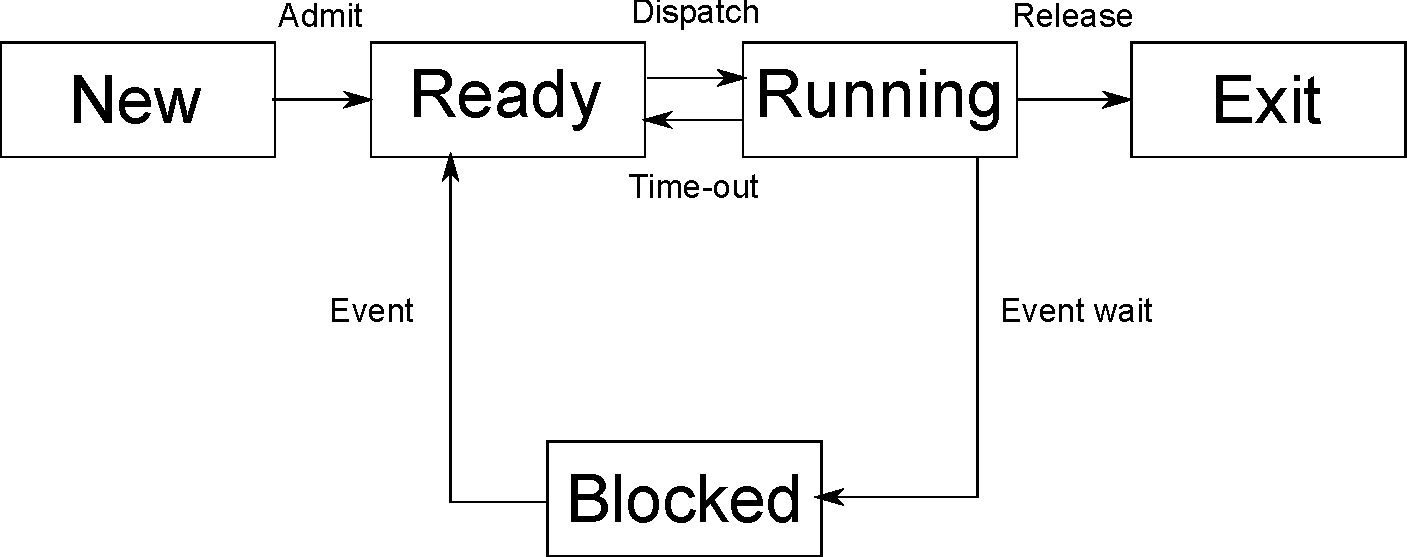
\includegraphics[width=\textwidth]{../images/StateSimple.pdf}
\end{frame}


\def\sectitle{Ordonnancement}
\subsection{\sectitle}
%%Frame
\begin{frame}{\sectitle}
%%Block
\def\subsectitle{Remarque}
\subsection{\subsectitle}
\begin{block}{\subsectitle}
\begin{itemize}
    \item Un processus choisi comment répartir son temps entre les threads qui
        le composent. 
\end{itemize}
\end{block}
%%Block
\def\subsectitle{Classe d'ordonancement}
\subsection{\subsectitle}
\begin{block}{\subsectitle}
\begin{itemize}
    \item Ancienneté (FIFO)
    \item Priorités (Fixes, variables)
    \item Quantum de temps durée max.
    \item Échéances
    \item Tourniquet
    \item Priorité et quantum
\end{itemize}
\end{block}
\end{frame}
\end{document}
